\subsection{Grid Computing}

Dupa cum se poate observa si din denumire, grid computing este format dintr-o retea de
calculatoarea care comunica intre ele printr-o interfata comuna. Deobicei interfata respectiva este
ethernet de viteze foate mari ( 10Gbps, 40 Gpbs sau chiar mai rapida), pentru a permite accesul de
la distanta. Grid computing este o ramura a retelelor distribuite, permitand folosirea resurselor
(computational sau stocare date), pentru a rezolva probleme complexe. Intr-un grid computing,
fiecare statie conectata la aceasta retea, are propriul sistem de operare, astfel, putand partaja
mai multe taskuri pentru a rula in paralel\cite{zhang2010comparison}.


\subsection{Cloud Computing}

Cloud computing nu are o definitie standard, numele parca fiind predestinat pentru acest tip de
situatie confuza. Cea mai des intalnita definitie a clodului este urmatoarea:

Cloud computing reprezinta o abstractizare a resurselor hardware, o virtualizare si o scalare
dinamica a lor pentru a putea pune la dispozitia clientilor resursele necesare in momentul
respectiv\cite{foster2008cloud}.

In figura 2.1 sunt prezentate tipurile de siteme distribuite. Se poate vedea faptul ca cloud
computing are la baza grid computing, mai bine zis,
cloud computing poate reprezenta o abstractizare a lui grid computing, deoarece nu trebuie sa sti
cate masini fizice ruleaza sau ce resurse se afla istalate pe ele, in cloud computing tot ce
conteaza e puterea totala necesara si resursele consumate (memoria ram sau spatiu de stocare). 


\begin{figure*}[ht] \centering
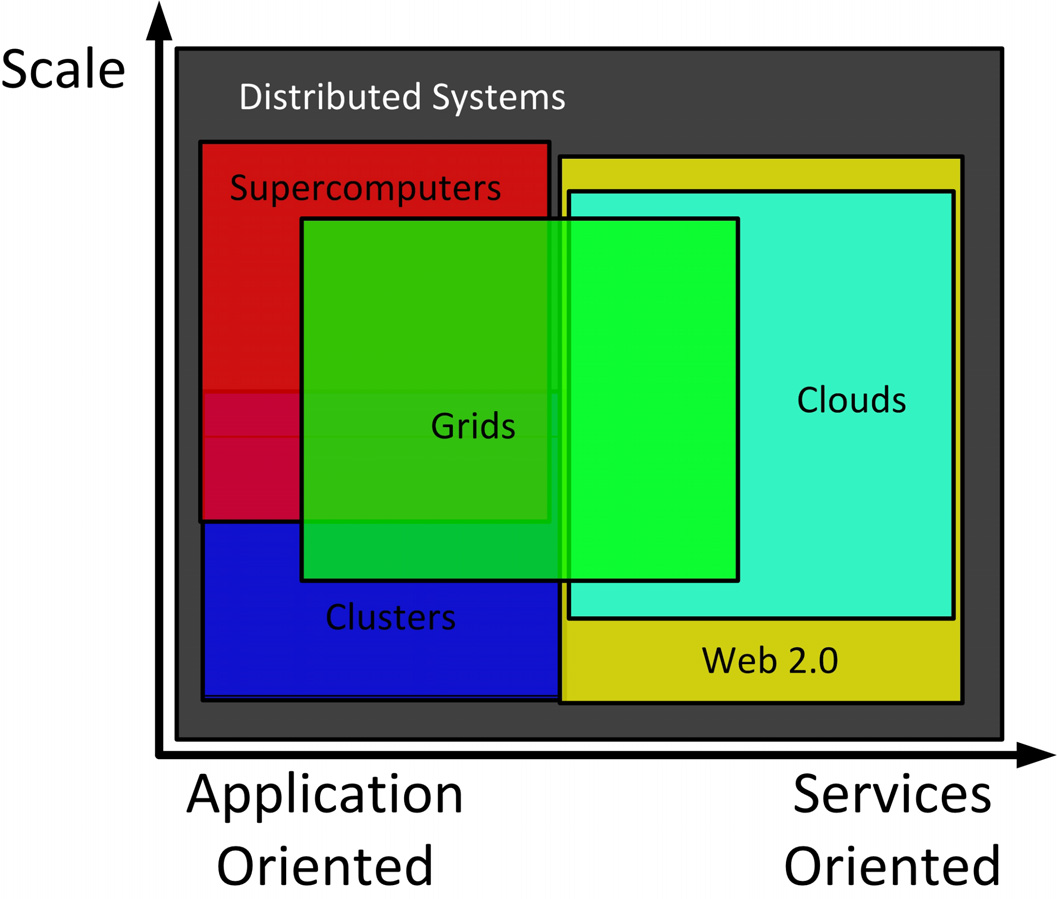
\includegraphics[width=0.6\textwidth]{img/clustergrid.png}
\caption{Tipurile de sisteme distribuite } \end{figure*}


